In this chapter, we present the basics of \amrex.  The implementation
source codes are in {\tt amrex/Src/Base/}.  Note that \amrex\ classes
and functions are in namespace {\tt amrex}.  For clarity, we usually
drop {\tt amrex::} in the example codes here.  It is also assumed that
headers have been properly {\tt include}d.  We recommend you study
the tutorial in {\tt amrex/Tutorials/Basic/HeatEquation\_EX1\_C} while reading this chapter.
After reading this chapter, one should be able to develop single-level
parallel codes using \amrex.  It should also be noted that this is not
a comprehensive reference manual.

\section{{\tt HeatEquation\_EX1\_C} Example}
The source code tree for the heat equation example is simple, as shown
in Figure \ref{fig:Basics_Heat_flowchart}.  We recommend you study
{\tt main.cpp} and {\tt advance.cpp} to see some of the classes described
below in action.
%%%%%%%%%%%%%%%%%%%%%%%%%%%%%
\begin{figure}[htb]
\begin{center}
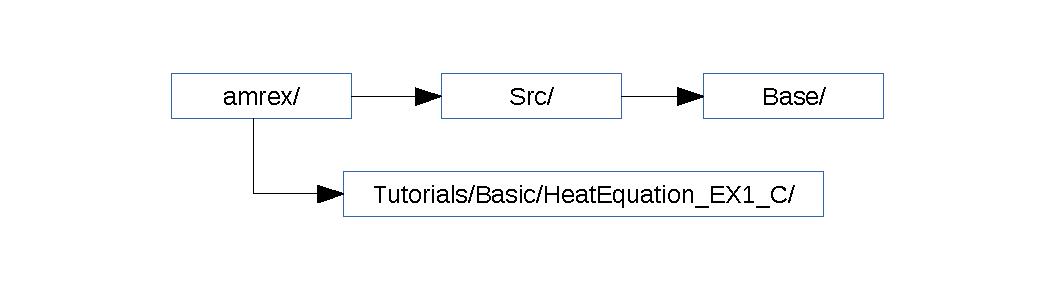
\includegraphics[width=4in]{./Basics/figs/flowchart.pdf}
\caption{\label{fig:Basics_Heat_flowchart} Source code tree for the 
         {\tt HeatEquation\_EX1\_C} example.}
\end{center}
\end{figure}
%%%%%%%%%%%%%%%%%%%%%%%%%%%%%
\begin{itemize}
\item {\tt Base/}\\
Contains source code for single-level \amrex simulations.
\item {\tt HeatEquation\_EX1\_C} \\
Build the code here by editing the {\tt GNUmakefile} and running {\tt make}.
\end{itemize}

\section{Dimensionality}
\label{sec:basics:dim}

As we have mentioned in Chapter~\ref{Chap:BuildingAMReX}, the
dimensionality of \amrex\ must be set at compile time.  A macro, {\tt
  AMREX\_SPACEDIM}, is defined to be the number of spatial
dimensions.  C++ codes can also use the {\tt amrex::SpaceDim}
variable.  Fortran codes can use either the macro and preprocessing or
do 
\begin{verbatim}
    use amrex_fort_module, only : amrex_spacedim
\end{verbatim}
The coordinate directions are zero based.

\section{Array}

{\tt Array} class in {\tt AMReX\_Array.H} is derived from {\tt
  std::vector}.  The only difference between {\tt Array} and {\tt
  std::vector} is that {\tt Array::operator[]} provides bound checking
when compiled with {\tt DEBUG=TRUE}.

\section{Real}

\amrex\ can be compiled to use either double precision (which is the
default) or single precision.  {\tt amrex::Real} is {\tt typedef}'d to
either {\tt double} or {\tt float}.  C codes can use {\tt
  amrex\_real}.  They are defined in {\tt AMReX\_REAL.H}.  The data
type is accessible in Fortran codes via
\begin{verbatim}
    use amrex_fort_module, only : amrex_real
\end{verbatim}

\section{ParallelDescriptor}
\label{sec:basics:paralleldescriptor}

\amrex\ users do not need to use MPI directly.  Parallel communication
is often handled by the data abstraction classes (e.g., {\tt
  MultiFab}; Section~\ref{sec:basics:multifab}).  In addition, \amrex\
has provided {\tt namespace ParallelDescriptor} in {\tt
  <AMReX\_ParallelDescriptor.H>}.  The frequently used functions are
\begin{lstlisting}[language=cpp]
 int myproc = ParallelDescriptor::MyProc();  // Return the rank
 
 int nprocs = ParallelDescriptor::NProcs();  // Return the number of processes
 
 if (ParallelDescriptor::IOProcessor()) { 
     // Only the I/O process executes this
 }
 
 int ioproc = ParallelDescriptor::IOProcessorNumber();  // I/O rank
 
 ParallelDescriptor::Barrier();
 
 // Broadcast 100 ints from the I/O Processor
 Array<int> a(100);
 ParallelDescriptor::Bcast(a.data(), a.size(),
                     ParallelDescriptor::IOProcessorNumber())
 
 // See AMReX_ParallelDescriptor.H for many other Reduce functions 
 ParallelDescriptor::ReduceRealSum(x);
\end{lstlisting}

\section{Print}
\label{sec:basics:print}

\amrex\ provides classes in {\tt AMReX\_Print.H} for printing messages
to standard output or any \cpp\ {\tt ostream}.  The main reason one
should use them instead of {\tt std::cout} is that messages from
multiple processes or threads do not get mixed up.  Below are some
examples.
\begin{lstlisting}[language=cpp]
 Print() <<  "x = " << x << "\n"; // Print on I/O processor
 
 Real pi = std::atan(1.0)*4.0;
 // Print on rank 3 with precision of 17 digits
 // SetPrecision does not modify cout's floating-point decimal precision setting.
 Print(3).SetPrecision(17) << pi << "\n";

 int oldprec = std::cout.precision(10);
 Print() << pi << "\n";  // Print with 10 digits
 
 AllPrint() << "Every process prints\n";  // Print on every process
 
 std::ofstream ofs("my.txt", std::ofstream::out);
 Print(ofs) << "Print to a file" << std::endl;
 ofs.close();
\end{lstlisting}

\section{ParmParse}
\label{sec:basics:parmparse}

{\tt ParmParse} in {\tt AMReX\_ParmParse.H} is a class providing a
database for the storage and retrieval of command-line and input-file
arguments.  When {\tt amrex::Initialize()} is called, the first
command-line argument after the executable name (if there is one and
it does not contain character {\tt =}) is taken to be the inputs file,
and the contents in the file are used to initialize the {\tt
  ParmParse} database.  The rest of the command-line arguments are
also parsed by {\tt ParmParse}.  The format of the inputs file is a
series of definitions in the form of {\tt prefix.name = value value
  ...}.  For each line, texts after {\tt \#} are comments.  Here is an
example inputs file.
\begin{quote}
\begin{verbatim}
nsteps    = 100               # integer
nsteps    = 1000              # nsteps appears a second time
dt        = 0.03              # floating point number
ncells    = 128 64 32         # a list of 3 ints
xrange    = -0.5 0.5          # a list of 2 reals
title     = "Three Kingdoms"  # a string
hydro.cfl = 0.8               # with prefix, hydro 
\end{verbatim}
\end{quote}
The following code shows how to use {\tt ParmParse} to get/query the values.
\begin{lstlisting}[language=cpp]
 ParmParse pp;
 
 int nsteps = 0;
 pp.query("nsteps", nsteps);
 amrex::Print() << nsteps << "\n";  // 1000
 
 Real dt;
 pp.get("dt", dt);  // runtime error if dt is not in inputs
 
 Array<int> numcells;
 // The variable name 'numcells' can be different from parameter name 'ncells'.
 pp.getarr("ncells", numcells);
 amrex::Print() << numcells.size() << "\n";  // 3
 
 Array<Real> xr {-1.0, 1.0};
 if (!queryarr("xrange", xr)) {
     amrex::Print() << "Cannot find xrange in inputs, "
                    << "so the default {-1.0,1.0} will be used\n";
 }
 
 std::string title;
 pp.query("title", title);  // query string
 
 ParmParse pph("hydro");  // with prefix 'hydro'
 Real cfl;
 pph.get("cfl", cfl);    // get parameter with prefix
\end{lstlisting}
Note that when there are multiple definitions for a parameter {\tt
  ParmParse} by default returns the last one.  The difference between
{\tt query} and {\tt get} should also be noted.  It is a runtime error
if {\tt get} fails to get the value, whereas {\tt query} returns an
error code without generating a runtime error that will abort the run.
If it is sometimes convenient to override parameters with command-line
arguments without modifying the inputs file.  The command-line
arguments after the inputs file are added later than the file to the
database and are therefore used by default.  For example, one can run
with
\begin{verbatim}
    myexecutable myinputsfile ncells="64 32 16" hydro.cfl=0.9
\end{verbatim}
to change the value of {\tt ncells} and {\tt hydro.cfl}.

\section{Example of AMR Grids}
\label{sec:basics:amrgrids}

In block-structured AMR, there is a hierarchy of logically rectangular
grids.  The computational domain on each AMR level is decomposed into
a union of rectangular domains.  Figure~\ref{fig:basics:amrgrids}
shows an example of AMR grids.  There are three total levels in the
example.  In \amrex\ numbering convention, the coarsest level is level
0.  The coarsest grid ({\emph{black}) covers the domain with $16^2$
cells. Bold lines represent grid boundaries.  There are two
intermediate resolution grids ({\emph{blue}}) at level 1 and the
cells are a factor of two finer than those at level 0.  The two finest
grids ({\emph{red}}) are at level 2 and the cells are a factor of two
finer than the level 1 cells.  Note that there is no direct
parent-child connection.  In this chapter, we will focus on single
levels.

\begin{figure}
  \centering
  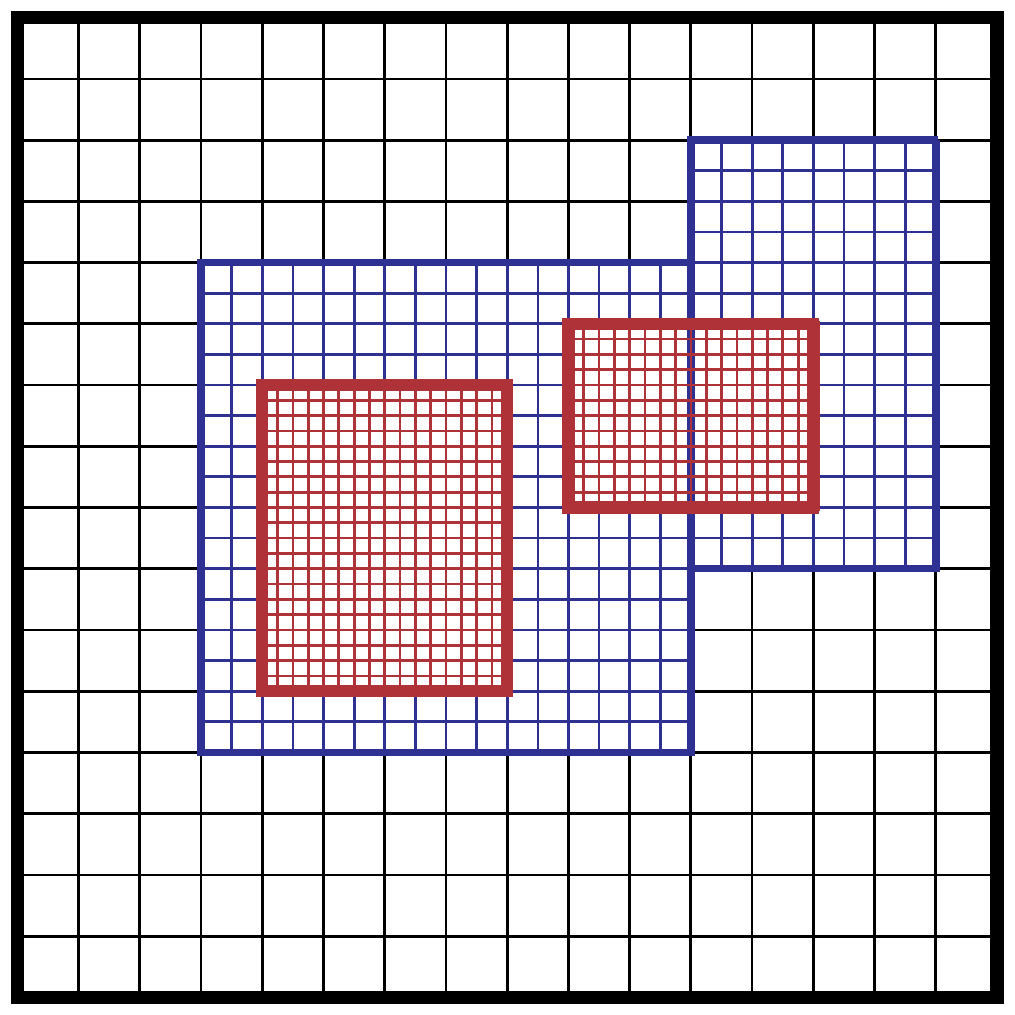
\includegraphics[width=3in]{./Basics/amrgrids.pdf}
  \caption{\label{fig:basics:amrgrids} Example of AMR grids.  There are
    three levels in total.  There are 1, 2 and 2 {\tt Box}es on levels
  0, 1, and 2, respectively.}
\end{figure}

\section{Box, IntVect and IndexType}
\label{sec:basics:box}

{\tt Box} in {\tt AMReX\_Box.H} is the data structure for representing
a rectangular domain in indexing space.  For example, in
Figure~\ref{fig:basics:amrgrids}, there are 1, 2 and 2 {\tt Box}es on
levels 0, 1 and 2, respectively.  {\tt Box} is a dimension dependent
class.  It has lower and upper corners (represented by {\tt IntVect}
and an index type (represented by {\tt IndexType}).  There are no
floating-point data in the object.

\subsection{IntVect}

{\idxamrex{IntVect}} is a dimension dependent class representing an
integer vector in {\idxamrex{AMREX\_SPACEDIM}}-dimensional space.  An
{\tt IntVect} can be constructed as follows,
\begin{lstlisting}[language=cpp]
 IntVect iv(AMREX_D_DECL(19, 0, 5));
\end{lstlisting}
Here {\tt AMREX\_D\_DECL} is a macro that expands {\tt
  AMREX\_D\_DECL(19,0,5)} to either {\tt 19} or {\tt 19,0} or {\tt
  19,0,5} depending on the number of dimensions.  The data can be
accessed via {\tt operator[]}, and the internal data pointer can be
returned by function {\tt getVect}.  For example
\begin{lstlisting}[language=cpp]
 for (int idim = 0; idim < AMREX_SPACEDIM; ++idim) {
     amrex::Print() << "iv[" << idim << "] = " << iv[idim] << "\n";
 }
 const int * p = iv.getVect();  // This can be passed to Fortran/C as an array
\end{lstlisting}

The class has a static function {\tt TheZeroVector()} returning the
zero vector, {\tt TheUnitVector()} returning the unit vector, and {\tt
  TheDimensionVector (int dir)} returning a reference to a constant
{\tt IntVect} that is zero except in the {\tt dir}-direction.  Note
the direction is zero-based.  {\tt IntVect} has a number of relational
operators, {\tt ==}, {\tt !=}, {\tt <}, {\tt <=}, {\tt >}, and {\tt
  >=} that can be used for lexicographical comparison (e.g., key of
{\tt std::map}), and a class {\tt IntVect::shift\_hasher} that can be
used as a hash function (e.g., for {\tt std::unordered\_map}).  It
also has various arithmetic operators.  For example,
\begin{lstlisting}[language=cpp]
 IntVect iv(AMREX_D_DECL(19, 0, 5));
 IntVect iv2((AMREX_D_DECL(4, 8, 0));
 iv += iv2;  // iv is now (23,8,5)
 iv *= 2;    // iv is now (46,16,10);
\end{lstlisting}

In AMR codes, one often needs to do refinement and coarsening on {\tt
  IntVect}.  The refinement operation can be done with the
multiplication operation.  However, the coarsening requires care
because of the rounding towards zero behavior of integer division in
Fortran, C and C++.  For example {\tt int i = -1/2} gives {\tt i =
  0}, and what we want is usually {\tt i = -1}.  Thus, one should use
the {\tt coarsen} functions:
\begin{lstlisting}[language=cpp]
  IntVect iv(AMREX_D_DECL(127,127,127));
  IntVect coarsening_ratio(AMREX_D_DECL(2,2,2));
  iv.coarsen(2);                 // Coarsen each component by 2
  iv.coarsen(coarsening_ratio);  // Component-wise coarsening
  const auto& iv2 = amrex::coarsen(iv, 2); // Return an IntVect w/o modifying iv
  IntVect iv3 = amrex::coarsen(iv, coarsening_return); // iv not modified
\end{lstlisting}

Finally, we note that {\tt operator<<} is overloaded for {\tt
  IntVect} and therefore one can call
\begin{lstlisting}[language=cpp]
  amrex::Print() << iv << "\n";
  std::cout << iv << "\n";
\end{lstlisting}

\subsection{IndexType}

This class defines an index as being cell based or node based in
each dimension.  The default constructor defines a cell based type in
all directions.  One can also construct an {\tt IndexType} with an
{\tt IntVect} with zero and one representing cell and node,
respectively.
\begin{lstlisting}[language=cpp]
 // Node in x-direction and cell based in y and z-directions
 // (i.e., x-face of numerical cells)
 IndexType xface(IntVect{AMREX_D_DECL(1,0,0)});
\end{lstlisting}
The class provides various functions including
\begin{lstlisting}[language=cpp]
 // True if the IndexType is cell based in all directions.
 bool cellCentered () const;

 // True if the IndexType is cell based in dir-direction.
 bool cellCentered (int dir) const;

 // True if the IndexType is node based in all directions.
 bool nodeCentered () const;

 // True if the IndexType is node based in dir-direction.
 bool nodeCentered (int dir) const;
\end{lstlisting}

Index type is a very important concept in \amrex.  It is a way of
representing the notion of indices $i$ and $i+1/2$.

\subsection{Box}

A {\tt Box} is an abstraction for defining discrete regions of {\tt
  AMREX\_SPACEDIM}-dimensional indexing space.  {\tt Box}es have an
{\tt IndexType} and two {\tt IntVect}s representing the lower and
upper corners.  Boxes can exist in positive and negative indexing
space.   Typical ways of defining a {\tt Box} are
\begin{lstlisting}[language=cpp]
 IntVect lo(AMREX_D_DECL(64,64,64));
 IntVect hi(AMREX_D_DECL(127,127,127));
 IndexType typ({AMREX_D_DECL(1,1,1)});
 Box cc(lo,hi);        // By default, Box is cell based.
 Box nd(lo,hi+1,typ);  // Construct a nodal Box.
 Print() << "A cell-centered Box " << cc << "\n";
 Print() << "An all nodal Box    " << nd << "\n";
\end{lstlisting}
Depending the dimensionality, the output of the code above is
\begin{verbatim}
  A cell-centered Box ((64,64,64) (127,127,127) (0,0,0))
  An all nodal Box    ((64,64,64) (128,128,128) (1,1,1))
\end{verbatim}
For simplicity, we will assume it is 3D for the rest of this section.
In the output, three integer tuples for each box are the lower corner
indices, upper corner indices, and the index types.  Note that {\tt 0}
and {\tt 1} denote cell and node, respectively.  For each tuple like
{\tt (64,64,64)}, the 3 numbers are for 3 directions.  The two {\tt
  Box}es in the code above represent different indexing views of the
same domain of $64^3$ cells.  Note that in \amrex\ convention, the
lower side of a cell has the same integer value as the cell centered
index.  That is if we consider a cell based index represent $i$, the
nodal index with the same integer value represents $i-1/2$.
Figure~\ref{fig:basics:indextypes} shows a 2D example of various index
types.  

\begin{figure}
  \centering
  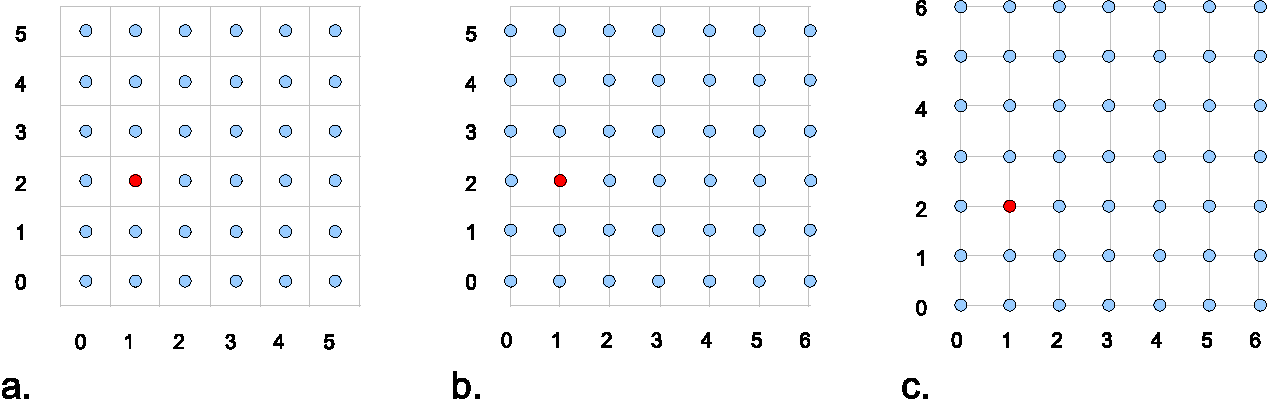
\includegraphics[width=5in]{./Basics/indextypes.pdf}
  \caption{\label{fig:basics:indextypes} Some of the different index
    types in two dimensions: (a) cell-centered, (b) $x$-face-centered
    (i.e., nodal in $x$-direction only), and (c) corner/nodal,
    i.e., nodal in all dimensions.}
\end{figure}

There are a number of ways of converting a {\tt Box} from one type to
another.
\begin{lstlisting}[language=cpp]
  Box b0 ({64,64,64}, {127,127,127}); // Index type: (cell, cell, cell)

  Box b1 = surroundingNodes(b0);  // A new Box with type (node, node, node)
  Print() << b1;                  // ((64,64,64) (128,128,128) (1,1,1))
  Print() << b0;                  // Still ((64,64,64) (127,127,127) (0,0,0))

  Box b2 = enclosedCells(b1);     // A new Box with type (cell, cell, cell)
  if (b2 == b0) {                 // Yes, they are identical.
     Print() << "b0 and b2 are identical!\n";
  }

  Box b3 = convert(b0, {0,1,0});  // A new Box with type (cell, node, cell)
  Print() << b3;                  // ((64,64,64) (127,128,127) (0,1,0))

  b3.convert({0,0,1});            // Convert b0 to type (cell, cell, node)
  Print() << b3;                  // ((64,64,64) (127,127,128) (0,0,1))

  b3.surroundingNodes();          //  Exercise for you
  b3.enclosedCells();             //  Exercise for you
\end{lstlisting}

The internal data of {\tt Box} can be accessed via various member functions.
Examples are
\begin{lstlisting}[language=cpp]
  const IntVect& smallEnd () const&;  // Get the small end of the Box
  int bigEnd (int dir) const;         // Get the big end in dir direction
  const int* loVect () const&;        // Get a const pointer to the lower end
  const int* hiVect () const&;        // Get a const pointer to the upper end
\end{lstlisting}

{\tt Box}es can be refined and coarsened.  Refinement or coarsening
does not change the index type.  Some examples are shown below.
\begin{lstlisting}[language=cpp]
  Box ccbx ({16,16,16}, {31,31,31});
  ccbx.refine(2);
  Print() << ccbx;                   // ((32,32,32) (63,63,63) (0,0,0))
  Print() << ccbx.coarsen(2);        // ((16,16,16) (31,31,31) (0,0,0))

  Box ndbx ({16,16,16}, {32,32,32}, {1,1,1});
  ndbx.refine(2);
  Print() << ndbx;                   // ((32,32,32) (64,64,64) (1,1,1))
  Print() << ndbx.coarsen(2);        // ((16,16,16) (32,32,32) (1,1,1))

  Box facebx ({16,16,16}, {32,31,31}, {1,0,0});
  facebx.refine(2);
  Print() << facebx;                 // ((32,32,32) (64,63,63) (1,0,0))
  Print() << facebx.coarsen(2);      // ((16,16,16) (32,31,31) (1,0,0))

  Box uncoarsenable ({16,16,16}, {30,30,30});
  print() << uncoarsenable.coarsen(2); // ({8,8,8}, {15,15,15});
  print() << uncoarsenable.refine(2);  // ({16,16,16}, {31,31,31});
                                       // Different from the original!
\end{lstlisting}
Note that refinement and coarsening behaviors depend on the indexing
type.  One should think the refinement and coarsening in AMR context
that refined or coarsened {\tt Box} still covers the same physical
domain.  {\tt Box uncoarsenable} in the example above is considered
uncoarsenable because its coarsened version does not cover the same
physical domain in the AMR context.

{\tt Box}es can grow and they can grow in all directions or just one
direction.  There are a number of {\tt grow} functions.  Some are
member functions of the {\tt Box} class and others are non-member
functions in the {\tt amrex} namespace. 

{\tt Box} class provides the following member functions testing if a {\tt
  Box} or {\tt IntVect} is contained within this {\tt Box}.  Note that
it is a runtime error if the two {\tt Box}es have different types.
\begin{lstlisting}[language=cpp]
  bool contains (const Box& b) const;
  bool strictly_contains (const Box& b) const;
  bool contains (const IntVect& p) const;
  bool strictly_contains (const IntVect& p) const;
\end{lstlisting}

Another very common operation is the intersection of two {\tt Box}es
like in the following examples.
\begin{lstlisting}[language=cpp]
  Box b0 ({16,16,16}, {31,31,31});
  Box b1 ({ 0, 0,30}, {23,23,63});
  if (b0.intersects(b1)) {                  // true
      Print() << "b0 and b1 intersect.\n"; 
  }

  Box b2 = b0 & b1;     // b0 and b1 unchanged
  Print() << b2;        // ((16,16,30) (23,23,31) (0,0,0))

  Box b3 = surroundingNodes(b0) & surroundingNodes(b1); // b0 and b1 unchanged
  Print() << b3;        // ((16,16,30) (24,24,32) (1,1,1))

  b0 &= b2;             // b2 unchanged
  Print() << b0;        // ((16,16,30) (23,23,31) (0,0,0))

  b0 &= b3;             // Runtime error because of type mismatch!
\end{lstlisting}

\section{RealBox and Geometry}

A {\tt RealBox} stores the physical location in floating-point numbers
of the lower and upper corners of a rectangular domain.

{\tt Geometry} class in {\tt AMReX\_Geometry.H} describes problem
domain and coordinate system for rectangular problem domains.  A {\tt
  Geometry} object can be constructed with
\begin{lstlisting}[language=cpp]
  explicit Geometry (const Box&     dom,
                     const RealBox* rb     = nullptr,
                     int            coord  = -1,
                     int*           is_per = nullptr);
\end{lstlisting}
Here the constructor takes a cell-centered {\tt Box} specifying the
indexing space domain, an optional argument of {\tt RealBox} pointer
specifying the physical domain, an optional {\tt int} specifying
coordinate system type, and an optional {\tt int*} specifying
periodicity.  If a {\tt RealBox} is not given, \amrex\ will construct
one based on {\tt ParmParse} parameters, {\tt geometry.prob\_lo} and
{\tt geometry.prob\_hi}, where each of the parameter is an array of
{\tt AMREX\_SPACEDIM} real numbers.  It's a runtime error if this
fails.  The optional argument for coordinate system is an integer type
with valid values being 0 (Cartesian), or 1 (cylindrical), or 2
(spherical).  If it is invalid as in the case of the default argument
value, \amrex\ will query the {\tt ParmParse} database for {\tt
  geometry.coord\_sys} and use it if one is found.  If it cannot find
the parameter, the coordinate system is set to 0 (i.e., Cartesian
coordinates).  {\tt Geometry} class has the concept of periodicity.
An optional argument can be passed specifying periodicity in each
dimension.  If it is not given, the domain is assumed to be
non-periodic unless there is the {\tt ParmParse} integer array
parameter {\tt geometry.is\_periodic} with {\tt 0} denoting
non-periodic and {\tt 1} denoting periodic.  Below is an example of
defining a {\tt Geometry} for a periodic rectangular domain of
$[-1.0,1.0]$ in each direction discretized with $64$ numerical cells
in each direction.
\begin{lstlisting}[language=cpp]
  int n_cell = 64;

  // This defines a Box with n_cell cells in each direction.
  Box domain(IntVect{AMREX_D_DECL(       0,        0,        0)},
             IntVect{AMREX_D_DECL(n_cell-1, n_cell-1, n_cell-1)});

  // This defines the physical box, [-1,1] in each direction.
  RealBox real_box({AMREX_D_DECL(-1.0,-1.0,-1.0)},
                   {AMREX_D_DECL( 1.0, 1.0, 1.0)});
  
  // This says we are using Cartesian coordinates
  int coord = 0;
  
  // This sets the boundary conditions to be doubly or triply periodic
  std::array<int,AMREX_SPACEDIM> is_periodic {AMREX_D_DECL(1,1,1)};
  
  // This defines a Geometry object
  Geometry geom(domain, &real_box, coord, is_periodic.data());
\end{lstlisting}

A {\tt Geometry} object can return various information of the physical
domain and the indexing space domain.  For example,
\begin{lstlisting}[language=cpp]
  const Real* problo = geom.ProbLo();    // Lower corner of the physical domain
  Real yhi = geom.ProbHi(1);             // y-direction upper corner
  const Real* dx = geom.CellSize();      // Cell size for each direction
  const Box& domain = geom.Domain();     // Index domain
  bool is_per = Geometry::isPeriodic(0); // Is periodic in x-direction?
  if (Geometry::isAllPeriodic()) {}      // Periodic in all direction?
  if (Geometry::isAnyPeriodic()) {}      // Periodic in any direction?
\end{lstlisting}


\section{BoxArray}
\label{sec:basics:ba}

{\tt BoxArray} is a class in {\tt AMReX\_BoxArray.H} for storing a
collection of {\tt Box}es on a single AMR level.  One can make a {\tt
  BoxArray} out of a single {\tt Box} and then chop it into multiple
{\tt Box}es.
\begin{lstlisting}[language=cpp]
  Box domain(IntVect{0,0,0}, IntVect{127,127,127});
  BoxArray ba(domain);  // Make a new BoxArray out of a single Box
  Print() << "BoxArray size is " << ba.size() << "\n";  // 1
  ba.maxSize(64);       // Chop into boxes of 64^3 cells
  Print() << ba;
\end{lstlisting}
The output is like below,
\begin{verbatim}
  (BoxArray maxbox(8)
         m_ref->m_hash_sig(0)
  ((0,0,0) (63,63,63) (0,0,0)) ((64,0,0) (127,63,63) (0,0,0))
  ((0,64,0) (63,127,63) (0,0,0)) ((64,64,0) (127,127,63) (0,0,0))
  ((0,0,64) (63,63,127) (0,0,0)) ((64,0,64) (127,63,127) (0,0,0))
  ((0,64,64) (63,127,127) (0,0,0)) ((64,64,64) (127,127,127) (0,0,0)) )
\end{verbatim}
It shows that {\tt ba} now has 8 {\tt Box}es, and it also prints out
each {\tt Box}.  

In \amrex, {\tt BoxArray} is a global data structure.  It holds all
the {\tt Box}es in a collection, even though a single process in a
parallel run only owns some of the {\tt Box}es via domain
decomposition.  In the example above, a 4-process run may divide the
work and each process owns say 2 {\tt Box}es
(Section~\ref{sec:basics:dm}).  Each process can then allocate memory
for the floating point data on the {\tt Box}es it owns
(Sections~\ref{sec:basics:multifab} \& \ref{sec:basics:fab}). 

{\tt BoxArray} has an indexing type, just like {\tt Box}.  Each {\tt
  Box} in a {\tt BoxArray} has the same type as the {\tt BoxArray}
itself.  In the following example, we show how one can convert {\tt
  BoxArray} to a different type. 
\begin{lstlisting}[language=cpp]
  BoxArray cellba(Box(IntVect{0,0,0}, IntVect{63,127,127}));
  cellba.maxSize(64);
  BoxArray faceba = cellba;       // Make a copy
  faceba.convert(IntVect{0,0,1}); // convert to index type (cell, cell, node)
  // Return an all node BoxArray
  const BoxArray& nodeba = amrex::convert(faceba, IntVect{1,1,1});
  Print() << cellba[0] << "\n";  // ((0,0,0) (63,63,63) (0,0,0))
  Print() << faceba[0] << "\n";  // ((0,0,0) (63,63,64) (0,0,1))  
  Print() << nodeba[0] << "\n";  // ((0,0,0) (64,64,64) (1,1,1))
\end{lstlisting}

As shown in the example above, {\tt BoxArray} has an {\tt operator[]}
that returns a {\tt Box} given an index.  It should be emphasized that
there is a difference between its behavior and the usual behavior of
an subscript operator one might expect.  The subscript operator in
{\tt BoxArray} returns by value instead of reference.  This means code
like below is meaningless because it modifies a temporary return
value. 
\begin{lstlisting}[language=cpp]
  ba[3].coarsen(2);  // DO NOT DO THIS!  Doesn't do what one might expect.
\end{lstlisting}

{\tt BoxArray} has a number of member functions that allow the {\tt
  Box}es to be modified.  For example,
\begin{lstlisting}[language=cpp]
  BoxArray& refine (int refinement_ratio);   // Refine each Box in BoxArray
  BoxArray& refine (const IntVect& refinement_ratio);
  BoxArray& coarsen (int refinement_ratio);  // Coarsen each Box in BoxArray
  BoxArray& coarsen (const IntVect& refinement_ratio);
\end{lstlisting}

We have mentioned at the beginning of this section that {\tt BoxArray}
is a global data structure storing {\tt Box}es shared by all processes.
The operation of a deep copy is thus undesirable because it
is expensive and the extra copy wastes memory.  The
implementation of the {\tt BoxArray} class uses {\tt std::shared\_ptr}
to an internal container holding the actual {\tt Box} data.  Thus
making a copy of {\tt BoxArray} is a quite cheap operation.  The
conversion of types and coarsening are also cheap because they can
share the internal data with the original {\tt BoxArray}.  In our
implementation, function
{\tt refine} does create a new deep copy of the original data.  Also
note that a {\tt BoxArray} and its variant with a different type share
the same internal data is an implementation detail.  We discuss this
so that the users are aware of the performance and resource cost.
Conceptually we can think of them as completely independent of each
other.
\begin{lstlisting}[language=cpp]
  BoxArray ba(...);  // original BoxArray
  BoxArray ba2 = ba; // a copy that shares the internal data with the original
  ba2.coarsen(2);    // Modify the copy
  // The original copy is unmodified even though they share internal data.
\end{lstlisting}

For advanced users, \amrex\ provides functions performing the
intersection of a {\tt BoxArray} and a {\tt Box}.  These functions are
much faster than a naive implementation of performing intersection of
the {\tt Box} with each {\tt Box} in the {\tt BoxArray}.  If one needs
to perform those intersections, functions {\tt amrex::intersect}, {\tt
  BoxArray::intersects} and {\tt BoxArray::intersections} should be
used.

\section{DistributionMapping}
\label{sec:basics:dm}

{\tt DistributionMapping} is a class in {\tt
  AMReX\_DistributionMapping.H} describes which process owns the data
living on the domains specified by the {\tt Box}es in a {\tt
  BoxArray}.  Like {\tt BoxArray}, there is an element for each {\tt
  Box} in {\tt DistributionMapping}, including the ones owned by other
parallel processes.  A way to construct a {\tt DistributionMapping}
object given a {\tt BoxArray} is as follows.
\begin{lstlisting}[language=cpp]
  DistributionMapping dm {ba};
\end{lstlisting}
Oftentimes what one needs is simply making a copy. 
\begin{lstlisting}[language=cpp]
  DistributionMapping dm {another_dm};
\end{lstlisting}
Note that this class is built using {\tt std::shared\_ptr}.  Thus
making a copy is relatively cheap in terms of performance and memory
resources.  This class has a subscript operator that returns the
process ID at a given index.

By default, {\tt DistributionMapping} uses an algorithm based on space
filling curve to determine the distribution.  One can change the default
via {\tt ParmParse} parameter {\tt DistributionMapping.strategy}.  {\tt
  KNAPSACK} is a common choice that is optimized for load balance.
One can also explicitly construct a distribution.
{\tt DistributionMapping} class allows the user to have complete control by
passing an array of integers. 
\begin{lstlisting}[language=cpp]
  DistributionMapping dm;   // empty object
  Array<int> pmap {...};
  // The user fills the pmap array with the values specifying owner processes
  dm.define(pmap);  // Build DistributionMapping given an array of process IDs.
\end{lstlisting}


\section{BaseFab, FArrayBox and IArrayBox}
\label{sec:basics:fab}

\amrex\ is a block-structured AMR framework.  Although AMR introduces
irregularity to the data and algorithms, there is regularity at the
block/{\tt Box} level due to rectangular domain, and the data structure
at the {\tt Box} level is conceptually simple.  {\tt BaseFab} is a
class template for multi-dimensional array-like data structure on a
{\tt Box}.  The template parameter is typically basic types such as
{\tt Real}, {\tt int} or {\tt char}.  The dimensionality of the array
is {\tt AMREX\_SPACEDIM} plus one.  The additional dimensional is for
the number of components.  The data are internally stored in a
contiguous block of memory in Fortran array order (i.e., column-major
order) for $(x,y,z,\mathrm{component})$, and each component also
occupies a contiguous block of memory because of the ordering.  For
example, a {\tt BaseFab<Real>} with 4 components defined on a
three-dimensional {\tt Box(IntVect\{-4,8,32\},IntVect\{32,64,48\})} is
like a Fortran array of {\tt real(amrex\_real),
  dimension(-4:32,8:64,32:48,0:3)}.  Note that the convention in \cpp\
part of \amrex\ is the component index is zero based.  The code for
constructing such an object is as follows,
\begin{lstlisting}[language=cpp]
  Box bx(IntVect{-4,8,32}, IntVect{32,64,48});
  int numcomps = 4;
  BaseFab<Real> fab(bx,numcomps);
\end{lstlisting}

Most applications do not use {\tt BaseFab} directly, but utilize
specialized classes derived from {\tt BaseFab}.  The most common types
are {\tt FArrayBox} in {\tt AMReX\_FArrayBox.H} derived from {\tt
  BaseFab<Real>} and {\tt IArrayBox} in {\tt AMReX\_IArrayBox.H}
derived from {\tt BaseFab<int>}.

These derived classes also obtain many {\tt BaseFab} member functions
via inheritance.  We now show some common usages of these functions.
To get the {\tt Box} where a {\tt BaseFab} or its derived object is
defined, one can call
\begin{lstlisting}[language=cpp]
  const Box& box() const;
\end{lstlisting}
To the number of component, one can call
\begin{lstlisting}[language=cpp]
  int nComp() const;
\end{lstlisting}
To get a pointer to the array data, one can call
\begin{lstlisting}[language=cpp]
  T* dataPtr(int n=0);     // Data pointer to the nth component
                           // T is template parameter (e.g., Real)
  const T* dataPtr(int n=0) const; // const version
\end{lstlisting}
The typical usage of the returned pointer is then to pass it to a
Fortran or C function that works on the array data (see
Section~\ref{sec:basics:fortran}).
{\tt BaseFab} has several functions that set the array data to a
constant value (e.g., 0).  Two examples are as follows.  
\begin{lstlisting}[language=cpp]
  void setVal(T x);        // Set all data to x
  // Set the sub-region specified by bx to value x starting from component
  // nstart.  ncomp is the total number of component to be set.
  void setVal(T x, const Box& bx, int nstart, int ncomp);
\end{lstlisting}
One can copy data from one {\tt BaseFab} to another.
\begin{lstlisting}[language=cpp]
  BaseFab<T>& copy (const BaseFab<T>& src, const Box& srcbox, int srccomp,
                    const Box& destbox, int destcomp, int numcomp);
\end{lstlisting}
Here the function copies the data from the region specified by {\tt
  srcbox} in the source {\tt BaseFab src} into the region specified by
{\tt destbox} in the destination {\tt BaseFab} that invokes the
function call.  Note that although {\tt srcbox} and {\tt destbox} may
be different, they must be the same size, shape and index type,
otherwise a runtime error occurs.  The user also specifies how many
components ({\tt int numcomp}) are copied starting at component {\tt
  srccomp} in {\tt src} and stored starting at component {\tt
  destcomp}.  {\tt BaseFab} has functions returning the minimum or
maximum value.
\begin{lstlisting}[language=cpp] 
  T min (int comp=0) const;  // Minimum value of given component.
  T min (const Box& subbox, int comp=0) const; // Minimum value of given 
                                               // component in given subbox.
  T max (int comp=0) const;  // Maximum value of given component.
  T max (const Box& subbox, int comp=0) const; // Maximum value of given 
                                               // component in given subbox.
\end{lstlisting}

{\tt BaseFab} also has many arithmetic functions.  Here are some
examples using {\tt FArrayBox}.
\begin{lstlisting}[language=cpp]
  Box box(IntVect{0,0,0}, IntVect{63,63,63});
  int ncomp = 2;
  FArrayBox fab1(box, ncomp);
  FArrayBox fab2(box, ncomp);
  fab1.setVal(1.0);    // Fill fab1 with 1.0
  fab1.mult(10.0, 0);  // Multiply component 0 by 10.0
  fab2.setVal(2.0);    // Fill fab2 with 2.0
  Real a = 3.0;
  fab2.saxpy(a, fab1); // For both components, fab2 <- a * fab1 + fab2
\end{lstlisting}
For more complicated expressions that not supported, one can write
Fortran or C functions for those (Section~\ref{sec:basics:fortran}).
Note that {\tt BaseFab} does provide operators for accessing the
data directly in \cpp.  For example, the {\tt saxpy} example above can
be done with
\begin{lstlisting}[language=cpp]
  // Iterate over all components
  for (int icomp=0; icomp < fab1.nComp(); ++icomp) {
      // Iterate over all cells in Box
      for (BoxIterator bit(fab1.box()); bit.ok(); ++bit) {
          // bit() returns IntVect
          fab2(bit(),icomp) = a * fab1(bit(),icomp) + fab2(bit(),icomp);
      }
  }
\end{lstlisting}
But this approach is generally not recommended for performance reason.
However, it can be handy for debugging.

{\tt BaseFab} and its derived classes are containers for data on {\tt
  Box}.  We recall that {\tt Box} has types
(Section~\ref{sec:basics:box}).  The examples in this section so far
use the default cell based type.  However, some functions will result
in a runtime error if the types mismatch.  For example.
\begin{lstlisting}[language=cpp]
  Box ccbx ({16,16,16}, {31,31,31});           // cell centered box
  Box ndbx ({16,16,16}, {31,31,31}, {1,1,1});  // nodal box
  FArrayBox ccfab(ccbx);
  FArrayBox ndfab(ndbx);
  ccfab.setVal(0.0);
  ndfab.copy(ccfab);   // runtime error due to type mismatch
\end{lstlisting}

Because it typically contains a lot of data, {\tt BaseFab}'s copy
constructor and copy assignment operator are disabled for performance
reason.  However, it does provide a move constructor.  In addition, it
also provides a constructor for making an alias of an existing
object.  Here is an example using {\tt FArrayBox}.
\begin{lstlisting}[language=cpp]
  FArrayBox orig_fab(box, 4);  // 4-component FArrayBox
  // Make a 2-component FArrayBox that is an alias of orig_fab
  // starting from component 1.
  FArrayBox alias_fab(orig_fab, amrex::make_alias, 1, 2);
\end{lstlisting}
In the example, the alias {\tt FArrayBox} has only two components even
though the original one has four components.  The alias has a sliced
component view of the original {\tt FArrayBox}.  This is possible
because of the array ordering.  It is however not possible to slice in
the real space (i.e., the first {\tt AMREX\_SPACEDIM} dimensions).
Note that no new memory is allocated in constructing the alias and the
alias contains a non-owning pointer.  It should be emphasized that the
alias will contain a dangling pointer after the original {\tt
  FArrayBox} reaches its end of life.

\section{FabArray, MultiFab and iMultiFab}
\label{sec:basics:multifab}

{\tt FabArray<FAB>} is a class template in {\tt AMReX\_FabArray.H} for
a collection of {\tt FAB}s on the same AMR level associated with a
{\tt BoxArray} (Section~\ref{sec:basics:ba}).  The template parameter
{\tt FAB} is usually {\tt BaseFab<T>} or its derived classes (e.g.,
{\tt FArrayBox}).  However, it can also be used to hold other data
structures.  To construct a {\tt FabArray}, a {\tt BoxArray} must be
provided because it is intended to hold {\emph{grid}} data defined on
a union of rectangular regions embedded in a uniform index space.  For
example, an {\tt FabArray} object can be used to hold data for one
level of the example grids of Figure~\ref{fig:basics:amrgrids}.

{\tt FabArray} is a parallel data structure that the data (i.e.,
{\tt FAB}) are distributed among parallel processes.  On each process,
the {\tt FabArray} contains only the {\tt FAB} objects owned by this
process, and the process operates only on its local data.  For
operations that require data owned by other processes, remote
communications are involved.  Thus, the construction of a {\tt
  FabArray} requires a {\tt DistributionMapping}
(Section~\ref{sec:basics:dm}) that specifies which process owns which
{\tt Box}.  For level 2 ({\emph{red}) in
Figure~\ref{fig:basics:amrgrids}, there are two {\tt Box}es.  Suppose
there are two parallel processes, and we use a {\tt
  DistributionMapping} that assigns one {\tt Box} to each process.
For {\tt FabArray} on each process, it is built on a {\tt BoxArray} with
2 {\tt Box}es, but contains only one {\tt FAB}.  

In \amrex, there are some specialized classes derived from {\tt
  FabArray}.  The {\tt iMultiFab} class in {\tt AMReX\_iMultiFab.H} is
derived from {\tt FabArray<IArrayBox>}.  The most commonly used {\tt
  FabArray} kind class is {\tt MultiFab} in {\tt AMReX\_MultiFab.H}
derived from {\tt FabArray<FArrayBox>}.  In the rest of this section,
we use {\tt MultiFab} as example.  However, these concepts are equally
applicable to other types of {\tt FabArray}s.  There are many ways to
define a {\tt MultiFab}.  For example,
\begin{lstlisting}[language=cpp]
  // ba is BoxArray
  // dm is DistributionMapping
  int ncomp = 4;
  int ngrow = 1;
  MultiFab mf(ba, mf, ncomp, ngrow);
\end{lstlisting}
Here we define a {\tt MultiFab} with 4 components and 1 ghost cell.  A
{\tt MultiFab} contains a number of {\tt FArrayBox}es
(Section~\ref{sec:basics:fab}) defined on {\tt Box}es grown by the
number of ghost cells (1 in this example).  That is the {\tt Box} in
the {\tt FArrayBox} is not exactly the same as in the {\tt BoxArray}.
If the {\tt BoxArray} has a {\tt Box\{(8,8,8) (15,15,15)\}}, the one
used for constructing {\tt FArrayBox} will be {\tt Box\{(7,7,7)
  (16,16,16)\}} in this example.  For cells in {\tt FArrayBox}, we
call those in the original {\tt Box} valid cells and the grown part
ghost cells.  Note that {\tt FArrayBox} itself alone does not have the
concept of ghost cell, whereas ghost cell is a key concept of {\tt
  MultiFab} that allows for local operations on ghost cell data
originated from remote processes.  We will discuss how to fill ghost
cells with data from valid cells later in this section.  {\tt
  MultiFab} also has a default constructor.  One can define an empty
{\tt MultiFab} first and then call the {\tt define} function as
follows.
\begin{lstlisting}[language=cpp]
  MultiFab mf;
  // ba is BoxArray
  // dm is DistributionMapping
  int ncomp = 4;
  int ngrow = 1;
  mf.define(ba, mf, ncomp, ngrow);
\end{lstlisting}
Given an existing {\tt MultiFab}, one can also make an alias {\tt
  MultiFab} as follows.
\begin{lstlisting}[language=cpp]
  // orig_mf is an existing MultiFab
  int start_comp = 3;
  int num_comps = 1;
  MultiFab alias_mf(orig_mf, amrex::make_alias, start_comp, num_comps);
\end{lstlisting}
Here the first integer parameter is the starting component in the
original {\tt MultiFab} that will become component 0 in the alias {\tt
  MultiFab} and the second integer parameter is the number of
components in the alias.  It's a runtime error if the sum of the two
integer parameters is greater than the number of the components in the
original {\tt MultiFab}.  Note that the alias {\tt MultiFab} has
exactly the same number of ghost cells as the original {\tt MultiFab}.

We often need to build new {\tt MultiFab}s that have the same {\tt
  BoxArray} and {\tt DistributionMapping} as a given {\tt MultiFab}.
Below is an example of how to achieve this.
\begin{lstlisting}[language=cpp]
  // mf0 is an already defined MultiFab
  const BoxArray& ba = mf0.boxArray();
  const DistributionMapping& dm = mf0.DistributionMap();
  int ncomp = mf0.nComp();
  int ngrow = mf0.nGrow();
  MultiFab mf1(ba,dm,ncomp,ngrow);  // new MF with the same ncomp and ngrow
  MultiFab mf2(ba,dm,ncomp,0);      // new MF with no ghost cells
  // new MF with 1 component and 2 ghost cells
  MultiFab mf3(mf0.boxArray(), mf0.DistributionMap(), 1, 2);               
\end{lstlisting}

As we have repeatedly mentioned in this chapter that {\tt Box} and
{\tt BoxArray} have various index types.  Thus, {\tt MultiFab} also
has an index type that is obtained from the {\tt BoxArray} used for
defining the {\tt MultiFab}.  It should be noted again that index type
is a very important concept in \amrex.  Let's consider an example of a
finite-volume code, in which the state is defined as cell averaged
variables and the fluxes are defined as face averaged variables.
\begin{lstlisting}[language=cpp]
  // ba is cell-centered BoxArray
  // dm is DistributionMapping
  int ncomp = 3;  // Suppose the system has 3 components
  int ngrow = 0;  // no ghost cells
  MultiFab state(ba, dm, ncomp, ngrow);
  MultiFab xflux(amrex::convert(ba, IntVect{1,0,0}), dm, ncomp, 0);
  MultiFab yflux(amrex::convert(ba, IntVect{0,1,0}), dm, ncomp, 0);
  MultiFab zflux(amrex::convert(ba, IntVect{0,0,1}), dm, ncomp, 0);
\end{lstlisting}
Here all {\tt MultiFab} use the same {\tt DistributionMapping}, but
their {\tt BoxArray}s have different index types.  The state is cell
based, whereas the fluxes are on the faces.  Suppose the cell based
{\tt BoxArray} contains a {\tt Box\{(8,8,16), (15,15,31)\}}.  The
state on that {\tt Box} is conceptually a Fortran Array with the
dimension of {\tt (8:15,8:15,16:31,0:2)}.  The fluxes are arrays with
slightly different indices.  For example, the $x$-direction flux for
that {\tt Box} has the dimension of {\tt (8:16,8:15,16:31,0:2)}.  Note
there is an extra element in $x$-direction.

The {\tt MultiFab} class provides many functions performing common
arithmetic operations on a {\tt MultiFab} or between {\tt MultiFab}s
built with the {\emph{same}} {\tt BoxArray} and {\tt DistributionMap}.
For example,
\begin{lstlisting}[language=cpp]
  Real dmin = mf.min(3);   // Minimum value in component 3 of MultiFab mf
                           // no ghost cells included
  Real dmax = mf.max(3,1); // Maximum value in component 3 of MultiFab mf
                           // including 1 ghost cell
  mf.setVal(0.0);          // Set all values to zero including ghost cells

  MultiFab::Add(mfdst, mfsrc, sc, dc, nc, ng);  // Add mfsrc to mfdst
  MultiFab::Copy(mfdst, mfsrc, sc, dc, nc, ng); // Copy from mfsrc to mfdst
  // MultiFab mfdst: destination 
  // MultiFab mfsrc: source
  // int      sc   : starting component index in mfsrc for this operation
  // int      dc   : starting component index in mfdst for this operation
  // int      sc   : number of components for this operation
  // int      ng   : number of ghost cells involved in this operation
  //                 mfdst and mfsrc may have more ghost cells
\end{lstlisting}
We refer the reader to {\tt Src/Base/AMReX\_MultiFab.H} and {\tt
  Src/Base/AMReX\_FabArray.H} for more details.  It should be noted
again it is a runtime error if the two {\tt MultiFab}s passed to functions
like {\tt MultiFab::Copy} are not built with the {\emph{same}} {\tt
  BoxArray} (including index type) and {\tt DistributionMapping}. 

It is usually the case that the {\tt Box}es in the {\tt BoxArray} used
for building a {\tt MultiFab} are non-intersecting except that they
can be overlapping due to nodal index type.  However, {\tt MultiFab}
can have ghost cells, and in that case {\tt FArrayBox}es are defined
on {\tt Box}es larger than the {\tt Box}es in the {\tt BoxArray}.
Parallel communication is then needed to fill the ghost cells with
valid cell data from other {\tt FArrayBox}es possibly on other
parallel processes.  The function for performing this type of
communication is {\tt FillBoundary}.
\begin{lstlisting}[language=cpp]
  MultiFab mf(...parameters omitted...);
  Geometry geom(...parameters omitted...);
  mf.FillBoundary();                    // Fill ghost cells for all components
                                        // Periodic boundaries are not filled.
  mf.FillBoundary(geom.periodicity());  // Fill ghost cells for all components
                                        // Periodic boundaries are filled.
  mf.FillBoundary(2, 3);        // Fill 3 components starting from component 2
  mf.FillBoundary(geom.periodicity(), 2, 3);
\end{lstlisting}
Note that {\tt FillBoundary} does not modify any valid cells.  Also
note that {\tt MultiFab} itself does not have the concept of
periodic boundary, but {\tt Geometry} has, and we can provide that
information so that periodic boundaries can be filled as well.  You
might have noticed that a ghost cell could overlap with multiple valid
cells from different {\tt FArrayBox}es in the case of nodal index
type.  In that case, it is unspecified that which valid cell's value
is used to fill the ghost cell.  It ought to be the case the values in
those overlapping valid cells are the same up to roundoff errors.

Another type of parallel communication is copying data from one {\tt
  MultiFab} to another {\tt MultiFab} with a different {\tt BoxArray}
or the same {\tt BoxArray} with a different {\tt
  DistributionMapping}.   The data copy is performed on the regions of
intersection.  The most generic interface for this is
\begin{lstlisting}[language=cpp]
  mfdst.ParallelCopy(mfsrc, compsrc, compdst, ncomp, ngsrc, ngdst, period, op);
\end{lstlisting}
Here {\tt mfdst} and {\tt mfsrc} are destination and source {\tt
  MultiFab}s, respectively.  Parameters {\tt compsrc}, {\tt compdst}, and {\tt
  ncomp} are integers specifying the range of components.  The copy is
performed on {\tt ncomp} components starting from component {\tt compsrc} of
{\tt mfsrc} and component {\tt compdst} of {\tt mfdst}.  Parameters {\tt
  ngsrc} and {\tt ngdst} specify the number of ghost cells involved for
the source and destination, respectively.  Parameter {\tt period} is
optional, and by default no periodic copy is performed.  Like {\tt
  FillBoundary}, one can use {\tt Geometry::periodicity()} to provide
the periodicity information.  The last parameter is also optional and
is set to {\tt FabArrayBase::COPY} by default.  One could also use
{\tt FabArrayBase::ADD}.  This determines whether the function copies
or adds data from the source to the destination.  Same as {\tt
  FillBoundary}, if a destination cell has multiple cells as source,
it is unspecified that which source cell is used.  This function has
two variants, in which the periodicity and operation type are also
optional.
\begin{lstlisting}[language=cpp]
  mfdst.ParallelCopy(mfsrc, period, op);  // mfdst and mfsrc must have the same
                                          // number of components
  mfdst.ParallelCopy(mfsrc, compsrc, compdst, ncomp, period, op);
\end{lstlisting}
Here the number of ghost cells involved is zero, and the copy is
performed on all components if unspecified (assuming the two {\tt
  MultiFab}s have the same number of components).  Similar to {\tt
  FillBoundary}, a destination cell may have multiple sources and
which source is used is unspecified.

\section{MFIter and Tiling}
\label{sec:basics:mfiter}

In this section, we will first show how {\tt MFIter} works without
tiling.  Then we will introduce the concept of logical tiling.
Finally we will show how logical tiling can be launched via {\tt
  MFIter}. 

\subsection{MFIter without Tiling}
\label{sec:basics:mfiter:notiling}

In Section~\ref{sec:basics:multifab}, we have shown some of the
arithmetic functionalities of {\tt MultiFab}, such as adding two {\tt
  MultiFab}s together.  In this section, we will show how you can
operate on the {\tt MultiFab} data with your own functions.  \amrex\
provides an iterator, {\tt MFIter} for looping over the {\tt
  FArrayBox}es in {\tt MultiFab}s.  For example,
\begin{lstlisting}[language=cpp]
  for (MFIter mfi(mf); mfi.isValid(); ++mfi) // Loop over grids
  {
      // This is the valid Box of the current FArrayBox.
      // By "valid", we mean the original ungrown Box in BoxArray.
      const Box& box = mfi.validbox();

      // A reference to the current FArrayBox in this loop iteration.
      FArrayBox& fab = mf[mfi];

      // Pointer to the floating point data of this FArrayBox.
      Real* a = fab.dataPtr();

      // This is the Box on which the FArrayBox is defined.
      // Note that "abox" includes ghost cells (if there are any),
      // and is thus larger than or equal to "box".
      const Box& abox = fab.box();

      // We can now pass the information to a function that does
      // work on the region (specified by box) of the data pointed to
      // by Real* a.  The data should be viewed as a multidimensional
      // with bounds specified by abox.
      // Function f1 has the signature of
      // void f1(const int*, const int*, Real*, const int*, const int*);
      f1(box.loVect(), box.hiVect(), a, abox.loVect(), abox.hiVect());
  }
\end{lstlisting}
Here function {\tt f1} is usually a Fortran subroutine with ISO C
binding interface like below,
\begin{lstlisting}[language=fortran]
  subroutine f1(lo, hi, a, alo, ahi) bind(c)
    use amrex_fort_module, only : amrex_real
    integer, intent(in) :: lo(3), hi(3), alo(3), ahi(3)
    real(amrex_real),intent(inout)::a(alo(1):ahi(1),alo(2):ahi(2),alo(3):ahi(3))
    integer :: i,j,k
    do     k = lo(3), hi(3)
      do   j = lo(2), hi(2)
        do i = lo(1), hi(1)
          a(i,j,k) = ...
        end do
      end do
    end do
  end subroutine f1
\end{lstlisting}
Here {\tt amrex\_fort\_module} is a Fortran module in \amrex\ and {\tt
  amrex\_real} is a Fortran kind parameter that matches {\tt
  amrex::Real} in \cpp.  In this example, we assume the spatial
dimension is 3.  In 2D, the function interface is different.  In
Section~\ref{sec:basics:fortran}, we will present a dimension agnostic
approach using macros provided by \amrex.

{\tt MFIter} only loops over grids owned by this process.  For
example, suppose there are 5 {\tt Box}es in total and processes 0 and
1 own 2 and 3 {\tt Box}es, respectively.  That is the {\tt MultiFab}
on process 0 has 2 {\tt FArrayBox}es, whereas there are 3 {\tt
  FArrayBox}es on process 1.  Thus the numbers of iterations of {\tt
  MFIter} are 2 and 3 on processes 0 and 1, respectively.

In the example above, {\tt MultiFab} is assumed to have a single
component.  If it has multiple component, we can call {\tt int nc =
  mf.nComp()} to get the number of components and pass it to the
kernel function.

There is only one {\tt MultiFab} in the example above.  Below is an
example of working with multiple {\tt MultiFab}s.  Note that these two
{\tt MultiFab}s are not necessarily built on the same {\tt BoxArray}.
But they must have the same {\tt DistributionMapping}, and their {\tt
  BoxArray}s are typically related (e.g., they are different due to
index types).
\begin{lstlisting}[language=cpp]
  // U and F are MultiFabs
  int ncU = U.nComp();   // number of components
  int ncF = F.nComp();
  for (MFIter mfi(F); mfi.isValid(); ++mfi) // Loop over grids
  {
      const Box& box = mfi.validbox();

      const FArrayBox& ufab = U[mfi];
      FArrayBox&       ffab = F[mfi];

      Real* up = ufab.dataPtr();
      Real* fp = ufab.dataPtr();

      const Box& ubox = ufab.box();
      const Box& fbox = ffab.box();

      // Function f2 has the signature of 
      // void f2(const int*, const int*,
      //         const Real*, const int*, const int*, const int*
      //               Real*, const int*, const int*, const int*);
      // This will compute f using u as inputs.
      f2(box.loVect(), box.hiVect(),
         up, ubox.loVect(), ubox.hiVect(), &ncU,
         fp, fbox.loVect(), fbox.hiVect(), &ncF);
  }
\end{lstlisting}
Here again function {\tt f2} is usually a Fortran subroutine with ISO
C binding interface like below,
\begin{lstlisting}[language=fortran]
subroutine f2(lo, hi, u, ulo, uhi, nu, f, flo, fhi, nf) bind(c)
  use amrex_fort_module, only : amrex_real
  integer, intent(in) :: lo(3),hi(3),ulo(3),uhi(3),nu,flo(3),fhi(3),nf
  real(amrex_real),intent(in   )::u(ulo(1):uhi(1),ulo(2):uhi(2),ulo(3):uhi(3),nu)
  real(amrex_real),intent(inout)::f(flo(1):fhi(1),flo(2):fhi(2),flo(3):fhi(3),nf)
  integer :: i,j,k
  do n = 1, nf
    do     k = lo(3), hi(3)
      do   j = lo(2), hi(2)
        do i = lo(1), hi(1)
          f(i,j,k,n) = ... u(...) ...
        end do
      end do
    end do
  end do
end subroutine f2
\end{lstlisting}

\subsection{MFIter with Tiling}
\label{sec:basics:mfiter:tiling}

Tiling, also known as cache blocking, is a well known loop
transformation technique for improving data locality.  This is often
done by transforming the loops into tiling loops that iterate over
tiles and element loops that iterate over the data elements within a
tile.  For example, the original loops might look like
\begin{lstlisting}[language=fortran]
  do k = kmin, kmax
    do j = jmin, jmax
      do i = imin, imax
        A(i,j,k) = B(i+1,j,k)+B(i-1,j,k)+B(i,j+1,k)+B(i,j-1,k) &
                  +B(i,j,k+1)+B(i,j,k-1)-6.0d0*B(i,j,k)
      end do
    end do
  end do
\end{lstlisting}
And the manually tiled loops might look like
\begin{lstlisting}[language=fortran]
  jblocksize = 11
  kblocksize = 16
  jblocks = (jmax-jmin+jblocksize-1)/jblocksize
  kblocks = (kmax-kmin+kblocksize-1)/kblocksize
  do kb = 0, kblocks-1
    do jb = 0, jblocks-1
      do k = kb*kblocksize, min((kb+1)*kblocksize-1,kmax)
        do j = jb*jblocksize, min((jb+1)*jblocksize-1,jmax)
          do i = imin, imax
            A(i,j,k) = B(i+1,j,k)+B(i-1,j,k)+B(i,j+1,k)+B(i,j-1,k) &
                      +B(i,j,k+1)+B(i,j,k-1)-6.0d0*B(i,j,k)
          end do
        end do
      end do
    end do
  end do
\end{lstlisting}
As we can see, to manually tile individual loops is very
labor-intensive and error-prone for large applications.  \amrex\ has
incorporated the tiling construct into {\tt MFIter} so that the
application codes can get the benefit of tiling easily.  An {\tt
  MFIter} loop with tiling is almost the same as the non-tiling
version.  The first example in
Section~\ref{sec:basics:mfiter:notiling} requires only two minor
changes: (1) passing {\tt true} when defining {\tt MFIter} to indicate
tiling; (2) calling {\tt tilebox} instead of {\tt validbox} to obtain
the work region for the loop iteration.
\begin{lstlisting}[language=cpp]
  //               * true *  turns on tiling
  for (MFIter mfi(mf,true); mfi.isValid(); ++mfi) // Loop over tiles
  {
      //                   tilebox() instead of validbox()
      const Box& box = mfi.tilebox();

      FArrayBox& fab = mf[mfi];
      Real* a = fab.dataPtr();
      const Box& abox = fab.box();

      f1(box.loVect(), box.hiVect(), a, abox.loVect(), abox.hiVect());
  }
\end{lstlisting}
The second example in Section~\ref{sec:basics:mfiter:notiling} also
requires only two minor changes.
\begin{lstlisting}[language=cpp]
  //              * true *  turns on tiling  
  for (MFIter mfi(F,true); mfi.isValid(); ++mfi) // Loop over tiles
  {
      //                   tilebox() instead of validbox()
      const Box& box = mfi.tilebox();

      const FArrayBox& ufab = U[mfi];
      FArrayBox&       ffab = F[mfi];

      Real* up = ufab.dataPtr();
      Real* fp = ufab.dataPtr();

      const Box& ubox = ufab.box();
      const Box& fbox = ffab.box();

      f2(box.loVect(), box.hiVect(),
         up, ubox.loVect(), ubox.hiVect(), &ncU,
         fp, fbox.loVect(), fbox.hiVect(), &ncF);
  }
\end{lstlisting}
The kernels functions like {\tt f1} and {\tt f2} in the two examples
here usually require very little changes.

\begin{figure}
  \centering
  \begin{minipage}{0.45\textwidth}
    \centering
    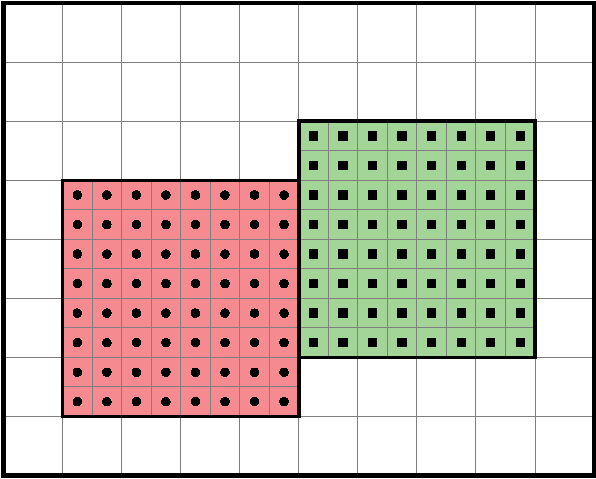
\includegraphics[width=0.9\textwidth]{./Basics/cc_validbox.pdf}
    \caption{\label{fig:basics:cc_validbox} Example of cell-centered valid boxes. There are two
    valid boxes in this example. Each has $8^2$ cells.}
  \end{minipage}\hfill
  \begin{minipage}{0.45\textwidth}
    \centering
    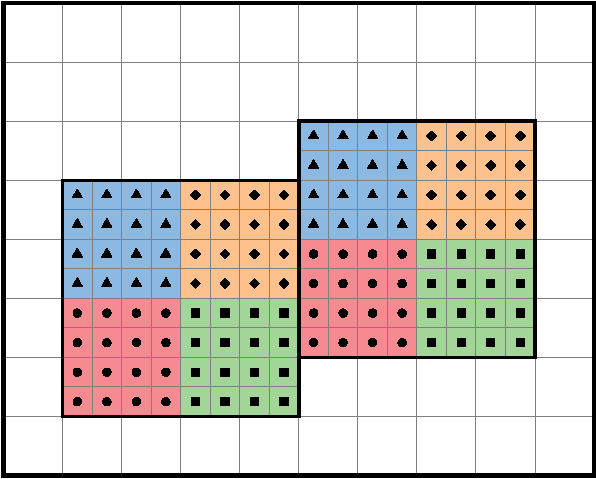
\includegraphics[width=0.9\textwidth]{./Basics/cc_tilebox.pdf}
    \caption{\label{fig:basics:cc_tilebox} Example of cell-centered tile boxes.
      Each grid is {\emph{logically}} broken into 4 tiles, and each
      tile has $4^2$ cells.  There are 8 tiles in total.}
  \end{minipage}
\end{figure}

Figures~\ref{fig:basics:cc_validbox} \& \ref{fig:basics:cc_tilebox}
show an example of the difference between {\tt validbox} and {\tt
  tilebox}.  In this example, there are two grids of cell-centered
index type.  Function {\tt validbox} always returns a {\tt Box} for the
valid region of an {\tt FArrayBox} no matter whether or not tiling is
enabled, whereas function {\tt tilebox} returns a {\tt Box} for a
tile.  (Note that when tiling is disabled, {\tt tilebox} returns the
same {\tt Box} as {\tt validbox}.)  The number of loop iteration is 2
in the non-tiling version, whereas in the tiling version the kernel
function is called 8 times.

The tile size can be explicitly set when defining {\tt MFIter}.
\begin{lstlisting}[language=cpp]
  // No tiling in x-direction. Tile size is 16 for y and 32 for z.
  for (MFIter mfi(mf,IntVect(1024000,16,32)); mfi.isValid(); ++mfi) {...}
\end{lstlisting}
An {\tt IntVect} is used to specify the tile size for every dimension.
A tile size larger than the grid size simply means tiling is disable
in that direction.  \amrex\ has a default tile size {\tt
  IntVect\{1024000,8,8\}} in 3D and no tiling in 2D.  This is used
when tile size is not explicitly set but the tiling flag is on.  One
can change the default size using {\tt ParmParse} parameter {\tt
  fabarray.mfiter\_tile\_size}.

\begin{figure}
  \centering
  \begin{minipage}{0.45\textwidth}
    \centering
    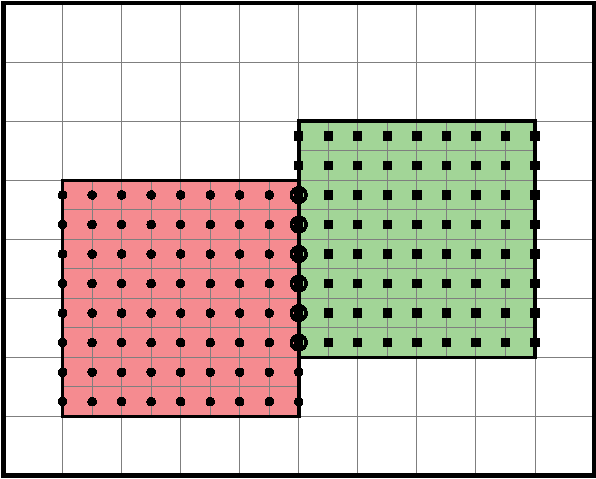
\includegraphics[width=0.9\textwidth]{./Basics/ec_validbox.pdf}
    \caption{\label{fig:basics:ec_validbox} Example of face valid
      boxes. There are two valid boxes in this example. Each has $9
      \times 8$ points.  Note that points in one {\tt Box} may overlap
      with points in the other {\tt Box}.  However, the memory locations
      for storing floating point data of those points do not overlap,
      because they belong to separate {\tt FArrayBox}es.}
  \end{minipage}\hfill
  \begin{minipage}{0.45\textwidth}
    \centering
    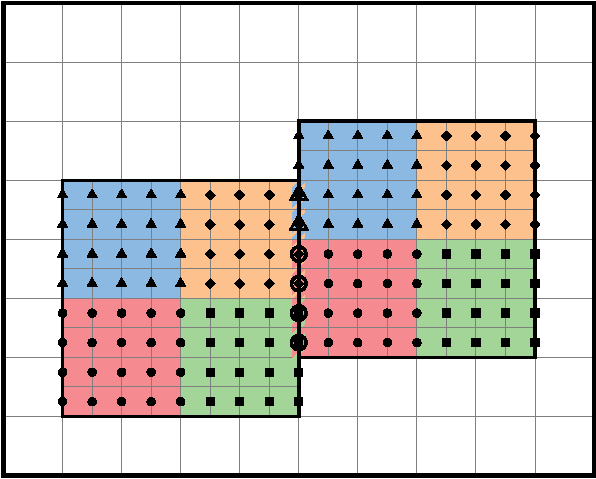
\includegraphics[width=0.9\textwidth]{./Basics/ec_tilebox.pdf}
    \caption{\label{fig:basics:ec_tilebox} Example of face tile boxes.
      Each grid is {\emph{logically}} broken into 4 tiles as indicated
      by the symbols.  There are 8 tiles in total.  Some tiles have $5
      \times 4$ points, whereas others have $4 \times 4$ points.
      Points from different {\tt Box}es may overlap, but points from
      different tiles of the same {\tt Box} do not.}
  \end{minipage}
\end{figure}

Usually {\tt MFIter} is used for accessing multiple {\tt MultiFab}s
like the second example, in which two {\tt MultiFab}s, {\tt U} and
{\tt F}, use {\tt MFIter} via {\tt operator []}.  These different {\tt
  MultiFab}s may have different {\tt BoxArray}s.  For example, {\tt U}
might be cell-centered, whereas {\tt F} might be nodal in
$x$-direction and cell in other directions.  The {\tt
  MFIter::validbox} and {\tt tilebox} functions return {\tt Box}es of
the same type as the {\tt MultiFab} used in defining the {\tt MFIter}
({\tt F} in this example).  Figures~\ref{fig:basics:ec_validbox} \&
\ref{fig:basics:ec_tilebox} show an example of non-cell-centered valid
and tile boxes.  Besides {\tt validbox} and {\tt tilebox}, {\tt
  MFIter} has a number of functions returning various {\tt Box}es.
Examples include,
\begin{lstlisting}[language=cpp]
  Box fabbox() const;       // Return the Box of the FArrayBox

  // Return grown tile box.  By default it grows by the number of
  // ghost cells of the MultiFab used for defining the MFIter.
  Box growntilebox(int ng=-1000000) const;

  // Return tilebox with provided nodal flag as if the MFIter
  // is constructed with MultiFab of such flag.
  Box tilebox(const IntVect& nodal_flag); 
\end{lstlisting} 
It should be noted that function {\tt growntilebox} does not grow the
tile {\tt Box} like a normal {\tt Box}.  Growing a {\tt Box} normally
means the {\tt Box} is extended in every face of every dimension.
However, function {\tt growntilebox} only extends the tile {\tt Box}
in such a way that tiles from the same grid do not overlap.  This is
the basic design principle of these various tiling functions.  Tiling
is a way of domain decomposition for work sharing.  Overlapping tiles
is undesirable because works would be wasted and for multi-threaded
codes race conditions could occur.
Figures~\ref{fig:basics:cc_growbox} \& \ref{fig:basics:ec_growbox}
show examples of {\tt growntilebox}.

\begin{figure}[t]
  \centering
  \begin{minipage}{0.45\textwidth}
    \centering
    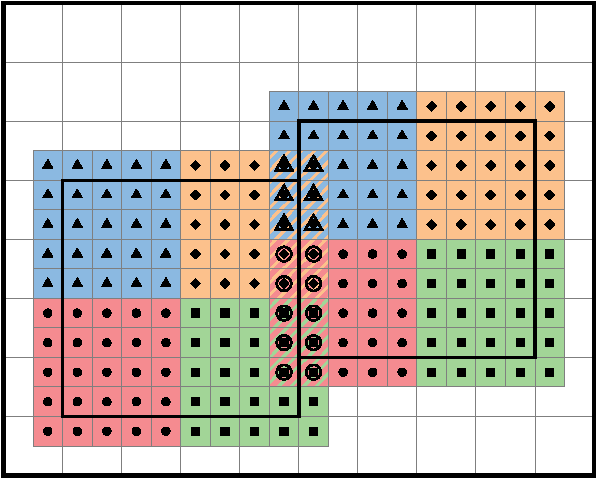
\includegraphics[width=0.9\textwidth]{./Basics/cc_growbox.pdf}
    \caption{\label{fig:basics:cc_growbox} Example of cell-centered
      grown tile boxes. As indicated by symbols, there are 8 tiles and
      four in each grid in this example. Tiles from the same grid do
      not overlap.  But tiles from different grids may overlap.}
  \end{minipage}\hfill
  \begin{minipage}{0.45\textwidth}
    \centering
    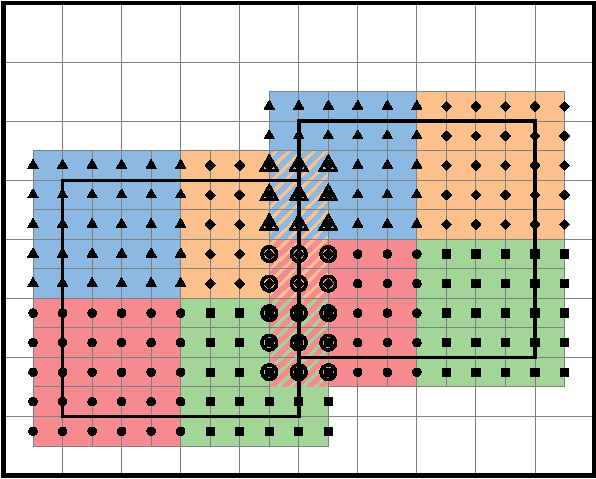
\includegraphics[width=0.9\textwidth]{./Basics/ec_growbox.pdf}
    \caption{\label{fig:basics:ec_growbox} Example of face type grown
      tile boxes.   As indicated by symbols, there are 8 tiles and
      four in each grid in this example. Tiles from the same grid do
      not overlap even though they have face index type. }
  \end{minipage}
\end{figure}

These functions in {\tt MFIter} return {\tt Box} by value.  There are
two ways of using these functions.
\begin{lstlisting}[language=cpp]
  const Box& bx = mfi.validbox();  // const& to temporary object is legal

  // Make a copy if Box needs to be modified later.
  // Compilers can optimize away the temporary object.
  Box bx2 = mfi.validbox();
  bx2.surroundingNodes();
\end{lstlisting}
But {\tt Box\& bx = mfi.validbox()} is not legal and will not compile.  

\section{Calling Fortran or C}
\label{sec:basics:fortran}

In Section~\ref{sec:basics:mfiter}, we have shown that a typical
pattern for working with {\tt MultiFab}s is use {\tt MFIter} to
iterate over the data.  In each iteration, a kernel function is called
to work on the data and the work region is specified by a {\tt Box}.
When tiling is used, the work region is a tile.  The tiling is logical
in the sense that there is no data layout transformation.  The kernel
function still gets the whole arrays in {\tt FArrayBox}es, even though
it is supposed to work on a tile region of the arrays.  To \cpp, these
kernel functions are C functions, whose function signatures are
typically declared in a header file named {\tt *\_f.H} or {\tt
  *\_F.H}.  We recommend the users to follow this convention.
Examples of these function declarations are as follows.
\begin{lstlisting}[language=cpp]
  #include <AMReX_BLFort.H>
  #ifdef __cplusplus
  extern "C"
  {
  #endif
      void f1(const int*, const int*, amrex_real*, const int*, const int*);
      void f2(const int*, const int*,
              const amrex_real*, const int*, const int*, const int*
              amrex_real*, const int*, const int*, const int*);
  #ifdef __cplusplus
  }
  #endif
\end{lstlisting}
One can write the functions in C and should include the header
containing the function declarations in the C source code to ensure
type safety.  However, we typically write these kernel functions in
Fortran because of the native multi-dimensional array support by
Fortran.  As we have seen in Section~\ref{sec:basics:mfiter}, these
Fortran functions take C pointers and view them as multi-dimensional
arrays of the shape specified by the additional integer arguments.
Note that Fortran takes arguments by reference unless the {\tt value}
keyword is used.  So an integer argument on the Fortran side matches
an integer pointer on the \cpp\ side.  Thanks to Fortran 2003,
function name mangling is easily achieved by declaring the Fortran
function as {\tt bind(c)}.

\amrex\ provides many macros for passing an {\tt FArrayBox}'s data
into Fortran/C.  For example
\begin{lstlisting}[language=cpp]
  for (MFIter mfi(mf,true); mfi.isValid(); ++mfi)
  {
      const Box& box = mfi.tilebox();
      f(BL_TO_FORTRAN_BOX(box),
        BL_TO_FORTRAN_ANYD(mf[mfi]));
  }
\end{lstlisting}
Here {\tt BL\_TO\_FORTRAN\_BOX} takes a {\tt Box} and provides two
{\tt int*}s specifying the lower and upper bounds of the {\tt Box}.
{\tt BL\_TO\_FORTRAN\_ANYD} takes an {\tt FArrayBox} returned by {\tt
  mf[mfi]} and the preprocessor turns it into {\tt Real*, int*, int*},
where {\tt Real*} is the data pointer that matches real array argument
in Fortran, the first {\tt int*} (which matches an integer argument in
Fortran) specifies the lower bounds, and the second {\tt int*} the
upper bounds of the spatial dimensions of the array.  Similar to what
we have seen in Section~\ref{sec:basics:mfiter}, a matching Fortran
function is shown below,
\begin{lstlisting}[language=fortran]
subroutine f(lo, hi, u, ulo, uhi) bind(c)
  use amrex_fort_module, only : amrex_real
  integer, intent(in) :: lo(3),hi(3),ulo(3),uhi(3)
  real(amrex_real),intent(inout)::u(ulo(1):uhi(1),ulo(2):uhi(2),ulo(3):uhi(3))
end subroutine f
\end{lstlisting}
Here, the size of the integer arrays is 3, the maximal number of
spatial dimensions.  If the actual spatial dimension is less than 3,
the values in the degenerate dimensions are set to zero.  So the
Fortran function interface does not have to change according to the
spatial dimensionality, and the bound of the third dimension of the
data array simply becomes {\tt 0:0}.  With the data passed by {\tt
  BL\_TO\_FORTRAN\_BOX} and {\tt BL\_FORTRAN\_ANYD}, this version of
Fortran function interface works for any spatial dimensions.  If one
wants to write a special version just for 2D and would like to use 2D
arrays, one can use
\begin{lstlisting}[language=fortran]
subroutine f2d(lo, hi, u, ulo, uhi) bind(c)
  use amrex_fort_module, only : amrex_real
  integer, intent(in) :: lo(2),hi(2),ulo(2),uhi(2)
  real(amrex_real),intent(inout)::u(ulo(1):uhi(1),ulo(2):uhi(2))
end subroutine f2d
\end{lstlisting}
Note that this does not require any changes in \cpp\ part, because
when \cpp\ passes an integer pointer pointing to an array of three
integers Fortran can treat it as a 2-element integer array.

Another commonly used macro is {\tt BL\_TO\_FORTRAN}.  This macro
takes an {\tt FArrayBox} and provides a real pointer for the floating
point data array and a number of integer scalars for the bounds.
However, the number of the integers depends on the dimensionality.
More specifically, there are 6 and 4 integers for 2D and 3D,
respectively.  The first half of the integers are the lower bounds for
each spatial dimension and the second half the upper bounds.  For
example,
\begin{lstlisting}[language=fortran]
subroutine f2d(u, ulo1, ulo2, uhi1, uhi2) bind(c)
  use amrex_fort_module, only : amrex_real
  integer, intent(in) :: ulo1, ulo2, uhi1, uhi2
  real(amrex_real),intent(inout)::u(ulo1:uhi1,ulo2:uhi2)
end subroutine f2d

subroutine f3d(u, ulo1, ulo2, ulo3, uhi1, uhi2, uhi3) bind(c)
  use amrex_fort_module, only : amrex_real
  integer, intent(in) :: ulo1, ulo2, ulo3, uhi1, uhi2, uhi3
  real(amrex_real),intent(inout)::u(ulo1:uhi1,ulo2:uhi2,ulo3:uhi3)
end subroutine f3d
\end{lstlisting}
Here for simplicity we have omitted passing the tile {\tt Box}.

Usually {\tt MultiFab}s have multiple components.  Thus we often also
need to pass the number of component into Fortran functions.  We can
obtain the number by calling the {\tt MultiFab::nComp()} function, and
pass it to Fortran as we have seen in Section~\ref{sec:basics:mfiter}.
We can also use the {\tt BL\_TO\_FORTRAN\_FAB} macro that is similar
to {\tt BL\_TO\_FORTRAN\_ANYD} except that it provides an additional
{\tt int*} for the number of components.  The Fortran function
matching {\tt BL\_TO\_FORTRAN\_FAB(fab)} is then like below,
\begin{lstlisting}[language=fortran]
subroutine f(u, ulo, uhi,nu) bind(c)
  use amrex_fort_module, only : amrex_real
  integer, intent(in) :: lo(3),hi(3),ulo(3),uhi(3),nu
  real(amrex_real),intent(inout)::u(ulo(1):uhi(1),ulo(2):uhi(2),ulo(3):uhi(3),nu)
end subroutine f
\end{lstlisting}

\section{Boundary}

\amrex\ uses {\tt MultiFab} as the data container for floating point
data on multiple {\tt Box}es on a single AMR level.  Each rectangular
{\tt Box} has its own boundaries.  A {\tt MultiFab} can have ghost cells for
storing data outside its grid {\tt Box} boundaries.  This allows us to
perform stencil type of operations on regular arrays.  There are three
basic types of boundaries: (1) interior boundary; (2) coarse/fine
boundary; and (3) physical boundary.  Periodic boundary is not
considered a basic type in the discussion here because after periodic
transformation it becomes either interior boundary or coarse/fine
boundary. 

Interior boundary is the border among the grid {\tt Box}es themselves.
For example, in Figure~\ref{fig:basics:amrgrids}, the two blue grid
{\tt Box}es on level 1 share an interior boundary that is 6 cells
long.  For a {\tt MultiFab} with ghost cells on level 1, we can use
the {\tt MultiFab::FillBoundary} function introduced in
Section~\ref{sec:basics:multifab} to fill ghost cells at the interior
boundary with valid cell data from other {\tt Box}es.

Coarse/fine boundary is the border between two AMR levels.  {\tt
FillBoundary} does not fill these ghost cells.  These ghost cells on
the fine level need to be interpolated from the coarse level data.
This is a subject that will be discussed in
Section~\ref{sec:amrcore:fillpatch}. 

The third type of boundary is the physical boundary at the physical
domain.  Note that both coarse and fine AMR levels could have grids
touching the physical boundary.  It is up to the application codes to
properly fill the ghost cells at the physical boundary.  However,
\amrex\ does provide support for some common operations.  To fill
ghost cells for cell-centered data at the physical boundary, we can
call
\begin{lstlisting}[language=cpp]
  void FillDomainBoundary (MultiFab& phi, const Geometry& geom,
                           const Array<BCRec>& bc);
\end{lstlisting}
Here we need to provide boundary types to each component of the {\tt
  MultiFab}.  Below is an example of setting up {\tt Array<BCRec>}
before the call.
\begin{lstlisting}[language=cpp]
  // Set up BC; see Src/Base/AMReX_BC_TYPES.H for supported types
  Array<BCRec> bc(phi.nComp());
  for (int n = 0; n < phi.nComp(); ++n)
  {
      for (int idim = 0; idim < AMREX_SPACEDIM; ++idim)
      {
          if (Geometry::isPeriodic(idim))
          {
              bc[n].setLo(idim, BCType::int_dir); // interior
              bc[n].setHi(idim, BCType::int_dir);
          }
          else
          {
              bc[n].setLo(idim, BCType::foextrap); // first-order extrapolation
              bc[n].setHi(idim, BCType::foextrap);
          }
      }
  }
\end{lstlisting}
{\tt amrex::BCType} has the following types,
\begin{quote}
\begin{description}
\item [int\_dir] Interior, including periodic boundary
\item [ext\_dir] It is the user's responsibility.
\item [foextrap] First order extrapolation from last cell in interior.
\item [reflect\_even] Reflection from interior cells with sign
  unchanged, $q(-i) = q(i)$.
\item [reflect\_odd] Reflection from interior cells with sign
  unchanged, $q(-i) = -q(i)$.
\end{description}
\end{quote}
If the type is set to {\tt BCType::ext\_dir}, it is then the user's
responsibility to fill the ghost cells.

\section{I/O}

In this section, we will discuss parallel I/O capabilities for mesh
data in \amrex.  Section~\ref{sec:Particles:IO} will discuss I/O for
particle data.

\subsection{Plotfile}

\amrex\ has its native plotfile format.  Many visualization tools are
available for \amrex\ plotfiles
(Chapter~\ref{Chap:Visualization}).  \amrex\ provides the following
two functions for writing a generic \amrex\ plotfile.  Many \amrex\
application codes may have their own plotfile routines that store
additional information such as compiler options, git hashes of the
source codes and {\tt ParmParse} runtime parameters.
\begin{lstlisting}[language=cpp]
  void WriteSingleLevelPlotfile (const std::string &plotfilename,
                                 const MultiFab &mf,
                                 const Array<std::string> &varnames,
                                 const Geometry &geom,
                                 Real time,
                                 int level_step);

  void WriteMultiLevelPlotfile (const std::string &plotfilename,
                                int nlevels,
                                const Array<const MultiFab*> &mf,
                                const Array<std::string> &varnames,
                                const Array<Geometry> &geom,
                                Real time,
                                const Array<int> &level_steps,
                                const Array<IntVect> &ref_ratio);
\end{lstlisting}
{\tt WriteSingleLevelPlotfile} is for single level runs and {\tt
WriteMultiLevelPlotfile} is for multiple levels.  The name of the
plotfile is specified by the {\tt plotfilename} argument.  This is the
top level directory name for the plotfile.  In \amrex\ convention, the
plotfile name consist of letters followed by numbers (e.g., {\tt
plt00258}).  {\tt amrex::Concatenate} is a useful helper function for
making such strings.
\begin{lstlisting}[language=cpp]
  int istep = 258;
  const std::string& pfname = amrex::Concatenate("plt",istep); // plt00258

  // By default there are 5 digits, but we can change it to say 4.
  const std::string& pfname2 = amrex::Concatenate("plt",istep,4); // plt0258  

  istep =1234567;  // Having more than 5 digits is OK.
  const std::string& pfname3 = amrex::Concatenate("plt",istep); // plt12344567
\end{lstlisting}
Argument {\tt mf} ({\tt MultiFab} for single level and {\tt
  Array<const MultiFab*>} for multi-level) is the data to be written
to the disk.  Note that many visualization tools expect this to be
cell-centered data.  So for nodal data, we need to convert them to
cell-centered data through some kind of averaging.  Also note that if
you have data at each AMR level in several {\tt MultiFab}s, you need
to build a new {\tt MultiFab} at each level to hold all the data on
that level.  This involves local data copy in memory and is not
expected to significantly increase the total wall time for writing
plotfiles.  For the multi-level version, the function expects {\tt
  Array<const MultiFab*>}, whereas the multi-level data are often
stored as {\tt Array<std::unique\_ptr<MultiFab>>}.  \amrex\ has a
helper function for this and one can use it as follows,
\begin{lstlisting}[language=cpp]
   WriteMultiLevelPlotfile(......, amrex::GetArrOfConstPtrs(mf), ......);
\end{lstlisting}
Argument {\tt varnames} has the names for each component of the {\tt
MultiFab} data.  The size of the {\tt Array} should be equal to the
number of components.  Argument {\tt geom} is for passing {\tt
Geometry} objects that contain the physical domain
information. Argument {\tt time} is for the time associated with the
data.  Argument {\tt level\_step} is for the current time step
associated with the data.  For multi-level plotfiles, argument {\tt
nlevels} is the total number of levels, and we also need to provide
the refinement ratio via an {\tt Array} of size {\tt nlevels-1}.

We note that \amrex\ does not overwrite old plotfiles if the new
plotfile has the same name.  The old plotfiles will be renamed to
new directories named like {\tt plt00350.old.46576787980}.

\subsection{Checkpoint File}

Checkpoint files are used for restarting simulations from where the
checkpoints are written.  Each application code has its own set of
data needed for restart.  \amrex\ provides I/O functions for basic
data structures like {\tt MultiFab} and {\tt BoxArray}.  These
functions can be used to build codes for reading and writing
checkpoint files.  Since each application code has its own
requirement, there is no standard \amrex\ checkpoint format.

Typically a checkpoint file is a directory containing some text files
and sub-directories (e.g., {\tt Level\_0} and {\tt Level\_1})
containing various data.  It is a good idea that we fist make these
directories ready for subsequently writing to the disk.  For example,
to build directories {\tt chk00016}, {\tt chk00016/Level\_0}, and {\tt
  chk00016/Level\_1}, we do
\begin{lstlisting}[language=cpp]
  const std::string& chkname {"chk00016"};
  const std::string& subDirPrefix {"Level_"};
  const int nSubDirs = 2;
  const bool callBarrier = true; // Parallel barrier after directories are built.
  PreBuildDirectorHierarchy(chkname, subDirPrefix, nSubDirs, callBarrier);
\end{lstlisting}

A checkpoint file of \amrex\ application codes often has a clear text
{\tt Header} file that only the I/O process writes to it using {\tt
std::ofstream}.  The {\tt Header} file contains information such as
the time, the physical domain size, grids, etc. that are necessary for
restarting the simulation.  To guarantee that precision is not lost
for storing floating point number like time in clear text file, the
file stream's precision needs to be set properly.  And a stream buffer
can also be used.  For example,
\begin{lstlisting}[language=cpp]
  if (ParallelDescriptor::IOProcessor())
  {
      const std::string& chkname = "chk00016";
      std::string HeaderFileName(chkname+"/Header");
      std::ofstream HeaderFile(HeaderFileName.c_str(),
           std::ofstream::out | std::ofstream::trunc | std::ofstream::binary);
      HeaderFile.precision(std::numeric_limits<Real>::max_digits10);
      VisMF::IO_Buffer io_buffer(VisMF::IO_Buffer_Size);
      HeaderFile.rdbuf()->pubsetbuf(io_buffer.dataPtr(), io_buffer.size());

      HeaderFile << "Checkpoint version 1.0\n";
      HeaderFile << time << "\n";
      HeaderFile << domain_box << "\n";
      // HeaderFile << ......;
      box_array.writeOn(HeaderFile); // write BoxArray
      // HeaderFile << ......;
  }
\end{lstlisting}
For reading the {\tt Header} file, \amrex\ can have the I/O process
read the file from the disk and broadcast it to others as {\tt
Array<char>}.  Then all processes can read the information with {\tt
std::istringstream}.  For example,
\begin{lstlisting}[language=cpp]
  std::string HeaderFileName {"chk00016/Header"};
  Array<char> fileChar;
  ParallelDescriptor::ReadAndBcastFile(HeaderFileName, fileChar);
  std::istringstream is(std::string{fileChar.data()}, std::istringstream::in);
  // is >> ....;
  BoxArray ba;
  ba.readFrom(is);
  // is >> ....;
\end{lstlisting}

{\tt amrex::VisMF} is a class that can be used to perform {\tt
  MultiFab} I/O in parallel.  How many processes are allowed to
perform I/O simultaneously can be set via
\begin{lstlisting}[language=cpp]
  VisMF::SetNOutFiles(64);  // up to 64 processes, which is also the default.
\end{lstlisting}
The optimal number is of course system dependent.  The following code
shows how to write and read a {\tt MultiFab}.
\begin{lstlisting}[language=cpp]
  const std::string name {"state"};

  VisMF::Write(mf, name);  // Write MultiFab to disk

  // Read the data to a new MultiFab
  // WARNING: mf2 may have a completely different DistributionMapping!
  MultiFab mf2;
  VisMF::Read(mf2, name);

  // Read the data to a MultiFab with identical
  // BoxArray, DistributionMapping, and number of components and ghost cells.
  MultiFab mf3(mf.boxArray(), mf.DistributionMap(), mf.nComp(), mf.nGrow());
  VisMF::Read(mf3, name);
\end{lstlisting}
It should be emphasized that calling {\tt VisMF::Read} with an empty
{\tt MultiFab} (i.e., no memory allocated for floating point data)
will result in a {\tt MultiFab} with a new {\tt DistributionMapping}
that could be different from any other existing {\tt
DistributionMapping} objects.  It should also be noted that all the
data including those in ghost cells are written/read by {\tt
VisMF::Write/Read}. 

\section{Memory Allocation}

\amrex\ has a Fortran module, {\tt mempool\_module} that can be used to
allocate memory for Fortran pointers.  The reason that such a module
exists in \amrex\ is memory allocation is often very slow in
multi-threaded OpenMP parallel regions.  \amrex\ {\tt mempool\_module}
provides a much faster alternative approach, in which each thread has
its own memory pool.  Here are examples of using the module.
\begin{lstlisting}[language=fortran]
  use mempool_module, only : bl_allocate, bl_deallocate
  real(amrex_real), pointer, contiguous :: a(:,:,:), b(:,:,:,:)
  integer :: lo1, hi1, lo2, hi2, lo3, hi3, lo(4), hi(4)
  ! lo1 = ...
  ! a(lo1:hi1, lo2:hi2, lo3:hi3)
  call bl_allocate(a, lo1, hi1, lo2, hi2, lo3, hi3)
  ! b(lo(1):hi(1),lo(2):hi(2),lo(3):hi(3),lo(4):hi(4))
  call bl_allocate(b, lo, hi)
  ! ......
  call bl_deallocate(a)
  call bl_deallocate(b)
\end{lstlisting}
The downside of this is we have to use {\tt pointer} instead of {\tt
allocatable}.  This means we must explicitly free the memory via {\tt
bl\_deallocate} and we need to declare the pointers as {\tt
contiguous} for performance reason.

\section{Abort and Assertion}

{\tt amrex::Abort(const char* message)} is used to terminate a run
usually when something goes wrong.  This function takes a message and
write it to stderr.  Files named like {\tt Backtrace.rg\_1\_rl\_1}
(where {\tt rg\_1\_rl\_1} means process 1) are produced containing
backtrace information of the call stack.  In Fortran, we can call {\tt
amrex\_abort} from the {\tt amrex\_error\_module}, which takes a
Fortran {\tt character} variable with assumed size (i.e., {\tt len=*})
as a message.

{\tt AMREX\_ASSERT} is a macro that takes a Boolean expression.  For
debug build (e.g., {\tt DEBUG=TRUE} using the GNU Make build system),
if the expression at runtime is evaluated to false, {\tt amrex::Abort}
will be called and the run is thus terminated.  For optimized build
(e.g., {\tt DEBUG=FALSE} using the GNU Make build system), the {\tt
AMREX\_ASSERT} statement is removed at compile time and thus has no
effect at runtime.  We often use this as a means of putting debug
statement in the code without adding any extra cost for production
runs.  For example,
\begin{lstlisting}[language=cpp]
  AMREX_ASSERT(mf.nGrow() > 0 && mf.nComp() == mf2.nComp());
\end{lstlisting}
Here for debug build we like to assert that {\tt MultiFab} {\tt mf}
has ghost cells and it also has the same number of components as {\tt
MultiFab} {\tt mf2}.  If we always want the assertion, we can use {\tt
AMREX\_ALWAYS\_ASSERT}.
